%%%%%%%%%%%%%%%%%%%%%%%%%%%%%%%%%%%%%%%%%%%%%%%%%%%%%%%%%%%%%%%%%%%%%%%%%%%
%% This file is part of the book
%%
%% Algorithmic Graph Theory
%% http://code.google.com/p/graph-theory-algorithms-book/
%%
%% Copyright (C) 2009, 2010 Minh Van Nguyen <nguyenminh2@gmail.com>
%%
%% See the file COPYING for copying conditions.
%%%%%%%%%%%%%%%%%%%%%%%%%%%%%%%%%%%%%%%%%%%%%%%%%%%%%%%%%%%%%%%%%%%%%%%%%%%

%% Chessboards with each square having dimensions 0.701125 x 0.701125.
%%
%% knight's initial position on 6 x 6 chessboard
\subfigure[A $6 \times 6$ chessboard.]{
\label{fig:graph_algorithms:reentrant_knight_tour:6_by_6_chessboard}
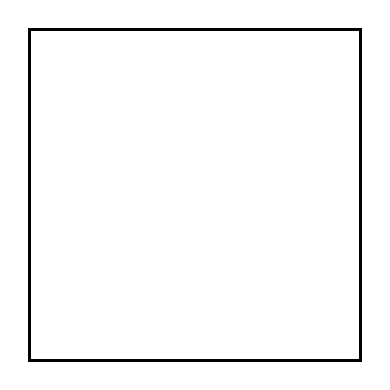
\begin{tikzpicture}
[borderdecorate/.style={-,very thick}]
%% chessboard with a black knight
\node at (0,3.5) {\WhiteEmptySquare\BlackEmptySquare\WhiteEmptySquare\BlackEmptySquare\WhiteEmptySquare\BlackEmptySquare};
\node at (0,2.8) {\BlackEmptySquare\WhiteEmptySquare\BlackEmptySquare\WhiteEmptySquare\BlackEmptySquare\WhiteEmptySquare};
\node at (0,2.1) {\WhiteEmptySquare\BlackEmptySquare\WhiteEmptySquare\BlackEmptySquare\WhiteEmptySquare\BlackEmptySquare};
\node at (0,1.4) {\BlackEmptySquare\WhiteEmptySquare\BlackEmptySquare\WhiteEmptySquare\BlackEmptySquare\WhiteEmptySquare};
\node at (0,0.7) {\WhiteEmptySquare\BlackEmptySquare\WhiteEmptySquare\BlackEmptySquare\WhiteEmptySquare\BlackEmptySquare};
\node at (0,0.0) {\BlackKnightOnBlack\WhiteEmptySquare\BlackEmptySquare\WhiteEmptySquare\BlackEmptySquare\WhiteEmptySquare};
%% the boarders of the chessboard
\draw[borderdecorate]
(-2.098875,-0.352) -- (-2.098875,3.85475) -- (2.107875,3.85475)
-- (2.107875,-0.352) -- cycle;
\end{tikzpicture}
}
\quad
%%
%% knight's tour
\subfigure[An $8 \times 8$ chessboard.]{
\label{fig:graph_algorithms:reentrant_knight_tour:8_by_8_chessboard}
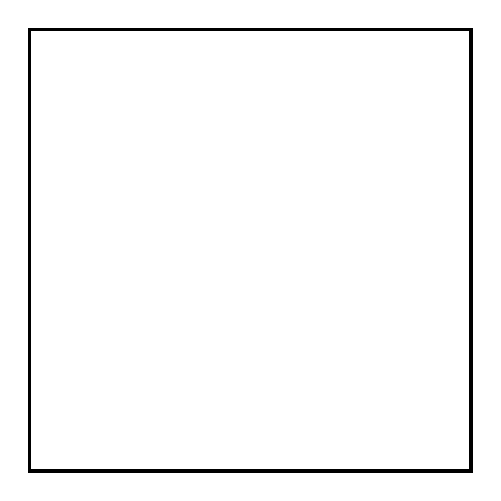
\begin{tikzpicture}
[borderdecorate/.style={-,very thick},%
  linedecorate/.style={-,thick},%
  nodedecorate/.style={shape=circle,fill=black,inner sep=2pt,draw,thick}]
%% empty chessboard
\node at (0,4.9) {\WhiteEmptySquare\BlackEmptySquare\WhiteEmptySquare\BlackEmptySquare\WhiteEmptySquare\BlackEmptySquare\WhiteEmptySquare\BlackEmptySquare};
\node at (0,4.2) {\BlackEmptySquare\WhiteEmptySquare\BlackEmptySquare\WhiteEmptySquare\BlackEmptySquare\WhiteEmptySquare\BlackEmptySquare\WhiteEmptySquare};
\node at (0,3.5) {\WhiteEmptySquare\BlackEmptySquare\WhiteEmptySquare\BlackEmptySquare\WhiteEmptySquare\BlackEmptySquare\WhiteEmptySquare\BlackEmptySquare};
\node at (0,2.8) {\BlackEmptySquare\WhiteEmptySquare\BlackKnightOnBlack\WhiteEmptySquare\BlackEmptySquare\WhiteEmptySquare\BlackEmptySquare\WhiteEmptySquare};
\node at (0,2.1) {\WhiteEmptySquare\BlackEmptySquare\WhiteEmptySquare\BlackEmptySquare\WhiteEmptySquare\BlackEmptySquare\WhiteEmptySquare\BlackEmptySquare};
\node at (0,1.4) {\BlackEmptySquare\WhiteEmptySquare\BlackEmptySquare\WhiteEmptySquare\BlackEmptySquare\WhiteEmptySquare\BlackEmptySquare\WhiteEmptySquare};
\node at (0,0.7) {\WhiteEmptySquare\BlackEmptySquare\WhiteEmptySquare\BlackEmptySquare\WhiteEmptySquare\BlackEmptySquare\WhiteEmptySquare\BlackEmptySquare};
\node at (0,0.0) {\BlackEmptySquare\WhiteEmptySquare\BlackEmptySquare\WhiteEmptySquare\BlackEmptySquare\WhiteEmptySquare\BlackEmptySquare\WhiteEmptySquare};
%% boarders of the chessboard
\draw[borderdecorate]
(-2.8,-0.352) -- (-2.8,5.257) -- (2.809,5.257) -- (2.809,-0.352) -- cycle;
\end{tikzpicture}
}
